% Created 2024-11-20 Wed 17:44
% Intended LaTeX compiler: lualatex
\documentclass[presentation,professionalfonts,aspectratio=169]{beamer}
                

% 
\makeatletter
 \@ifclassloaded{beamer}{%
  %%% save beamer's `solution' environment as `beamersolution':
  \let\beamersolution\solution
  \let\endbeamersolution\endsolution
  %%% "delete" the `solution' environment:
  \let\solution\relax
  \let\endsolution\relax
}{%
}%
\makeatother
\usepackage[utf8]{inputenc}
\usepackage[T1]{fontenc}
%\usepackage[french]{babel}
\usepackage[portuguese]{babel}

%%%% FONTS




\usepackage{xsim}
\usepackage[most]{tcolorbox}
\usepackage{amssymb}
\usepackage{fontawesome}
\newcounter{paragraph}



\DeclareExerciseEnvironmentTemplate{custom}{%
  \begin{tcolorbox}[boxrule = 0pt]
  \tcbox[on line,colback=teal,colframe=teal,coltext=white,size=small]{%
    \faBook\sffamily\bfseries\
    \XSIMmixedcase{\GetExerciseName}
    \GetExerciseProperty{counter}%
  }\quad
}{\end{tcolorbox}}


\DeclareExerciseEnvironmentTemplate{custom2}{%
  \begin{tcolorbox}[boxrule = 0pt]
  \tcbox[on line,colback=violet,colframe=violet,coltext=white,size=small]{%
    \faToggleOn\sffamily\bfseries\
    \XSIMmixedcase{\GetExerciseName}
    \GetExerciseProperty{counter}%
  }\quad
}{\end{tcolorbox}}




\DeclareExerciseType{test}{
	exercise-env = question ,
	solution-env = answer ,
	exercise-template = custom ,
	solution-template = custom2 ,
	exercise-name	= Exemplo. ,
	exercises-name = Exemplo ,
	solution-name = Solução ,
	solutions-name = Sol. ,
	exercise-heading = \textbf ,
	solution-heading = \textbf
}


\xsimsetup{
  exercise/within = section,
  exercise/the-counter =  \arabic{exercise}, 
%%solution-name = solution,  % used with headings=true
solution/print=false,
%print-collection/print=both,
}





\usepackage{colortbl}
\usepackage[tikz]{bclogo}
\usetikzlibrary{fit,patterns,shadows.blur,shapes,mindmap}
\usetikzlibrary{arrows,calc,arrows.meta,decorations.markings,shapes.symbols}
\usetikzlibrary{decorations.pathreplacing, decorations.pathmorphing,calc,arrows,positioning}
\usepackage{tikzpeople}
\usepackage{qrcode,hyperref}
\usepackage{upgreek}
%\usepackage[version=4]{mhchem}
\usepackage{tabularray}


\NewTblrTheme{fancy}{
\SetTblrStyle{caption-tag}{font=\bfseries}
\SetTblrInner[tblr,longtblr]{rowsep=2.5pt}
\DefTblrTemplate{firsthead, middlehead,lasthead}{default}{} % <---
\DefTblrTemplate{contfoot-text}{normal}{\scriptsize\textit{Continued on the next page}}
\SetTblrTemplate{contfoot-text}{normal}
}






\usepackage{chemfig,chemmacros,elements,chemformula}
\chemsetup{modules={all}}
\chemsetup[redox]{pos=top,roman=false}
\chemsetup[redox]{pos=top}
\chemsetup{redox/sep=.5em}
\chemsetup[redox]{explicit-sign=true}
\NewChemPhase\lqdd{\(\ell\)}
\NewChemPhase\gr{grafite}
\NewChemPhase\reac{reação}
\NewChemState\Enthalpy{symbol=H,superscript=,unit=\kilo\joule}%
\usepackage{siunitx}
\setchemfig{fixed length=false, atom sep=2.5em, arrow offset=6pt, scheme debug=false}%,angle increment=30}
\renewcommand*\printatom[1]{\ensuremath{\mathsf{#1}}} % This line changes the font of the atoms to sans serif
%%%% QRCODE
\usepackage{pdfpages}
\usepackage{mol2chemfig}
\usepackage{subfig,caption}
\usepackage{wrapfig}
\usepackage{enumitem}
\setitemize{label=\usebeamerfont*{itemize item}%
\usebeamercolor[fg]{itemize item}
\usebeamertemplate {itemize item}}
\usepackage{array} % ajust colunm table
\usepackage{cancel}
\usepackage[controls]{animate}
\renewcommand{\CancelColor}{\color{red}}

%%%%%%%%%%%%%%%%%%% CONFIG TCOLORBOX 

\newtcolorbox{mybox}[2][]{boxsep=0.5em,left=0.5em,
colback=blue!5!white, colframe=blue!75!black,
fonttitle=\bfseries\sffamily,
colbacktitle=blue!85!red!60,enhanced,
attach boxed title to top left={yshift=-3mm,xshift=5mm},
title=#2,#1}

\newtcolorbox{myrule}[2][]{boxsep=0.5em,left=0.5em,
colback=green!5!white, colframe=blue!75!black,
fonttitle=\bfseries\sffamily,
colbacktitle=blue!85!red!60,enhanced,
attach boxed title to top left={yshift=-3mm,xshift=5mm},
title=#2,#1}


\newtcolorbox{myex}[2][]{boxsep=0.5em,left=0.5em,
  colback=yellow!5!white, colframe=blue!75!black, 
  fonttitle=\bfseries\sffamily,
  colbacktitle=blue!85!red!60,enhanced,
  attach boxed title to top left={yshift=-3mm,xshift=5mm},
  title=#2,#1}


 \definecolor{col1}{HTML}{FF7878}
 \definecolor{col2}{HTML}{51B5F8}
 \definecolor{col3}{HTML}{68E1AA}
 \definecolor{col4}{HTML}{B869EA}
 \definecolor{col5}{HTML}{FF5500}
 \definecolor{col6}{HTML}{FFF8E7}
 \definecolor{col7}{HTML}{FF9966}
 \definecolor{col8}{HTML}{9400D3}



\definesubmol\nobond{-[,0.2,,,draw=none]\scriptstyle\color{blue}}
\newcommand{\re}{\hspace{-1cm}}
\newcommand{\af}{\hspace{2cm}}

%%%% Config X sim for BEAMER
\usepackage{ragged2e}
\justifying
\makeatletter
\@ifclassloaded{beamer}{%
%%% save beamer's `solution' environment as `beamersolution':
\let\beamersolution\solution
\let\endbeamersolution\endsolution
%%% "delete" the `solution' environment:
\let\solution\relax
\let\endsolution\relax
}{%
}%
\makeatother
\usepackage[utf8]{inputenc}
\usepackage[T1]{fontenc}
%\usepackage[portuguese, ]{babel}
%%%% FONTS
%%% XSIM CONFIG BEAMER
\usepackage{xsim}
\usepackage{amsmath}
\usepackage[most]{tcolorbox}
\usepackage{amssymb}
\usepackage{fontawesome}
\usepackage{tasks}
\newcounter{paragraph}
%\usepackage[dvipsnames,svgnames]{xcolor}
\usepackage[dvipsnames]{xcolor}
\usepackage{annotate-equations}
%%% BOX EXERCISE BEAMER
\DeclareExerciseEnvironmentTemplate{custom}{%
\begin{tcolorbox}[boxrule = 0pt]
\tcbox[on line,colback=teal,colframe=teal,coltext=white,size=small]{%
\faBook\sffamily\bfseries\
\XSIMmixedcase{\GetExerciseName}
\GetExerciseProperty{counter}%
}\quad
}{\end{tcolorbox}}
%% == CUSTOM BOX BEAMER
\DeclareExerciseEnvironmentTemplate{custom2}{%
\begin{tcolorbox}[boxrule = 0pt]
\tcbox[on line,colback=violet,colframe=violet,coltext=white,size=small]{%
\faToggleOn\sffamily\bfseries\
\XSIMmixedcase{\GetExerciseName}
\GetExerciseProperty{counter}%
}\quad
}{\end{tcolorbox}}
\DeclareExerciseType{test}{
exercise-env = question ,
solution-env = answer ,
exercise-template = custom ,
solution-template = custom2 ,
exercise-name = Exemplo ,
exercises-name = Exemplo ,
solution-name = Solução ,
solutions-name = Sol. ,
exercise-heading = \textbf ,
solution-heading = \textbf
}
\xsimsetup{
exercise/within = section,
exercise/the-counter =  \arabic{exercise},
%%solution-name = solution,  % used with headings=true
solution/print=true,
print-collection/print=both,
}
\NewTasksEnvironment[label = (\emph{\alph*}),
label-width = 12pt]{choice}[\choice]
\usepackage{empheq} %%% Brackers
\usepackage{colortbl}
\usepackage[tikz]{bclogo}
\usetikzlibrary{calc,fadings,shadings}
\usetikzlibrary{fit,patterns,shadows.blur,shapes,mindmap}
\usetikzlibrary{arrows,snakes,shapes,arrows.meta,decorations.markings,shapes.symbols}
\usetikzlibrary{backgrounds,shapes.geometric}
\usetikzlibrary{decorations.pathreplacing, decorations.pathmorphing,arrows,positioning}
\usepackage{tikzpeople}
\usepackage{qrcode,hyperref}
\usepackage{upgreek}
%\usepackage[version=4]{mhchem}
\usepackage{tabularray}
%%% PACKAGE PLOT GRAPH
\usepackage{pgfplots}
\pgfplotsset{width=10cm,compat=1.9}
%%% CUSTOM TABLE
\NewTblrTheme{fancy}{
\SetTblrStyle{caption-tag}{font=\bfseries,red2}
\SetTblrInner[tblr,longtblr]{rowsep=2.5pt}
\DefTblrTemplate{firsthead, middlehead,lasthead}{default}{} % <---
\DefTblrTemplate{contfoot-text}{normal}{\scriptsize\textit{Continua ...}}
\SetTblrTemplate{contfoot-text}{normal}
}
%% ==== CHEMMACROS E CHEMFIG CONFIG
\usepackage{chemfig,chemmacros,elements,chemformula}
\chemsetup{modules={all}}
\chemsetup[redox]{pos=top,roman=false}
\chemsetup[redox]{pos=top}
\chemsetup{redox/sep=.5em}
\chemsetup[redox]{explicit-sign=true} %%% reaction redox
%% == CUSTOM PHASES IN CHEMMACROS
\NewChemPhase\lqdd{\(\ell\)}
\NewChemPhase\gr{grafite}
\NewChemPhase\reac{reação}
\NewChemState\Enthalpy{symbol=H,superscript=,unit=\kilo\joule}%
\usepackage{siunitx}
\setchemfig{fixed length=false, atom sep=2.5em, arrow offset=6pt, scheme debug=false}
%% == NUMEROS PARA FORMULES
\renewcommand*\printatom[1]{\ensuremath{\mathsf{#1}}} % This line changes the font of the atoms to sans serif
%%% INCLUDE PAGES PDFs
\usepackage{pdfpages}
\usepackage{mol2chemfig}
\usepackage{xymtexpdf}
%\changeunitlength{0.08pt}
%%\wedgehasheddash
\usepackage{subfig,caption}
\usepackage{wrapfig}
\usepackage{enumitem}
\setitemize{label=\usebeamerfont*{itemize item}%
\usebeamercolor[fg]{itemize item}
\usebeamertemplate {itemize item}}
\usepackage{array} % ajust colunm table
\usepackage{cancel}
\usepackage[controls]{animate}
\usepackage{movie15}
\renewcommand{\CancelColor}{\color{red}}
%%%%%%%%%%%%%%%%%%% CONFIG TCOLORBOX
\newtcolorbox{mybox}[2][]{boxsep=0.5em,left=0.5em,
colback=blue!5!white, colframe=blue!75!black,
fonttitle=\bfseries\sffamily,
colbacktitle=blue!85!red!60,enhanced,
attach boxed title to top left={yshift=-3mm,xshift=5mm},
title=#2,#1}
\newtcolorbox{myrule}[2][]{boxsep=0.5em,left=0.5em,
colback=green!5!white, colframe=blue!75!black,
fonttitle=\bfseries\sffamily,
colbacktitle=blue!85!red!60,enhanced,
attach boxed title to top left={yshift=-3mm,xshift=5mm},
title=#2,#1}
\newtcolorbox{myex}[2][]{boxsep=0.5em,left=0.5em,
colback=yellow!5!white, colframe=blue!75!black,
fonttitle=\bfseries\sffamily,
colbacktitle=blue!85!red!60,enhanced,
attach boxed title to top left={yshift=-3mm,xshift=5mm},
title=#2,#1}
\tcbset{colback=yellow!10!white, colframe=red!50!black, highlight math style= {enhanced, %<-- needed for the ’remember’ options
colframe=red,colback=red!10!white,boxsep=0pt}}
\definecolor{col1}{HTML}{FF7878}
\definecolor{col2}{HTML}{51B5F8}
\definecolor{col3}{HTML}{68E1AA}
\definecolor{col4}{HTML}{B869EA}
\definecolor{col5}{HTML}{FF5500}
\definecolor{col6}{HTML}{FFF8E7}
\definecolor{col7}{HTML}{FF9966}
\definecolor{col8}{HTML}{9400D3}
%% CONFIG COLOR CARBONO
\tikzstyle{bal}=[inner sep=0.3pt,fill=orange,fill opacity=0.5,circle,minimum size=0.2cm]
\tikzstyle{rect}=[inner sep=0.3pt,fill=red,fill opacity=0.5,circle,minimum size=0.2cm]
\tikzstyle{bal2}=[inner sep=0.3pt,fill=blue,fill opacity=0.5,circle,minimum size=0.2cm]
\tikzstyle{bal3}=[inner sep=0.3pt,fill=yellow,fill opacity=0.5,circle,minimum size=0.2cm]
\definesubmol\nobond{-[,0.2,,,draw=none]\scriptstyle\color{blue}}
\newcommand{\re}{\hspace{-1cm}}
\newcommand{\af}{\hspace{2cm}}
\tikzstyle{mybox} = [draw=red, fill=blue!20, very thick, rectangle, rounded corners, inner sep=10pt, inner ysep=20pt]
\tikzstyle{fancytitle} =[fill=red, text=white]
\date{}
%\usetheme{minflat}
\usetheme{minflat}
\author{Fábio Lima}
\date{}
\title{ Isomeria Óptica}
\hypersetup{
 pdfauthor={Fábio Lima},
 pdftitle={ Isomeria Óptica},
 pdfkeywords={},
 pdfsubject={},
 pdfcreator={Emacs 29.4 (Org mode 9.6.15)}, 
 pdflang={En Portuguese}}
\begin{document}

\begingroup
  \setbeamertemplate{headline}{}
  \maketitle
  \endgroup
\begin{frame}{Sumário}
\tableofcontents
\end{frame}



\section{Isomeria Óptica}
\label{sec:orgb9bf24b}

\begin{frame}[label={sec:orgc648da3}]{Isomeria Óptica}
\begin{itemize}
\item Tipo de isomeria em que uma molécula é a imagem especular da outra.
\item Ocorre em moléculas que não apresentam plano de simetria (moléculas assimétricas).
\item \alert{Isômeros Óticos} ou \alert{Enantiomorfos} ou \alert{Enantiômeros}
\end{itemize}

\begin{bclogo}[couleur=blue!30 , arrondi=0.1 , logo=\bcplume , epBarre=3.5]{Definição}
\alert{Estereoisômeros} são substâncias que têm a mesma sequência de átomos ligados, mas que se diferenciam no arranjo espacial dos átomos. Eles também são chamados de isômeros configuracionais.
\end{bclogo}
\end{frame}


\begin{frame}[label={sec:org08c99e6}]{}
\begin{itemize}
\item Esta molécula não apresenta nenhum plano de simetria.
\item É denominada molécula assimétrica ou molécula \alert{quiral}.
\item Se a colocarmos diante de um espelho, a imagem especular será diferente dela.
\end{itemize}
\end{frame}

\begin{frame}[label={sec:org6944305}]{}
\begin{center}
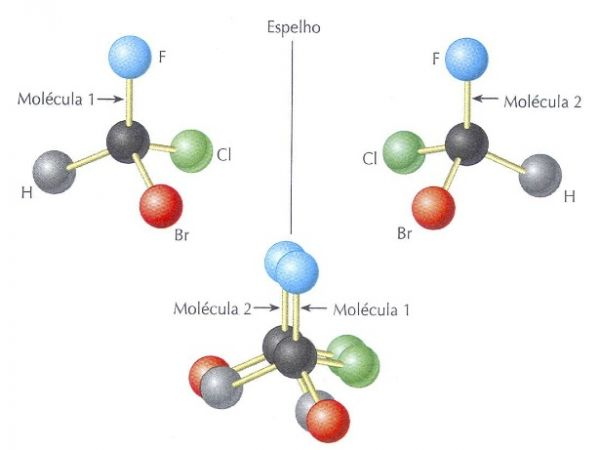
\includegraphics[scale=.45]{QO/Isomeria/Isomeria_Espelho.jpg}
\end{center}
\end{frame}



\section{Carbono Quiral}
\label{sec:orgda921eb}

\begin{frame}[label={sec:org2e8935c}]{Carbono Quiral}
\begin{itemize}
\item Condição para haver isômeros óticos: presença de carbono \alert{quiral} ou \alert{assimétrico}
\end{itemize}

\begin{bclogo}[couleur=yellow!30 , arrondi=0.1 , logo=\bcplume , epBarre=3.5]{}
\begin{center}
	\resetchemfig
	\schemestart
	\chemfig{R_2-@{a1}\textcolor{red}{C}([:90]-R_1)([:-90]-R_3)-R_4} \qquad \qquad 	\arrow 	\chemfig{Br-\textcolor{red}{C}([:90]-F)([:-90]-NH_2)-OH}
	\schemestop
	\chemmove{
	\node (text) [draw=none, font=\bfseries] at (-8,2){Carbono Quiral};
	\draw[red,shorten <=2pt,shorten >=1pt] (text) -- (a1) {};
	}
\end{center}
R1, R2, R3 e R4 são todos ligantes diferentes 
\end{bclogo}
\end{frame}



\begin{frame}[label={sec:orgc521007}]{Compostos oticamente ativos}
\begin{itemize}
\item Exemplo açúcares, incluindo a \alert{sacarose.} \textcolor{red}{$*$} Este asterisco sinaliza os carbonos assimétricos.
\end{itemize}


\begin{columns}
\begin{column}{0.4\columnwidth}
    \scriptsize
\schemestart
	\resetchemfig	\chemname{\chemfig{[2]CH_2@{a1}OH@{a2}-C\rlap{\large\textcolor{red}{*}}(-[4]H)([0]-@{a3}OH@{a4})-C\rlap{\large\textcolor{red}{*}}(-[4]H)([0]-@{a5}OH@{a6})-C\rlap{\large\textcolor{red}{*}}(-[4]@{a7}HO@{a8})([0]-H)-C\rlap{\large\textcolor{red}{*}}(-[4]H)([0]-@{a9}OH@{a10})-@{AA1}C(=[1]@{AA1a}O)(-[3]H)@{AA2}}}{Glicose}
	 %\arrow{0}[2,0]
	\schemestop
	\chemmove{
	\tikzstyle{colorir1}=[circle,inner sep=1pt,fill=ForestGreen,fill opacity=0.5,]
	\tikzstyle{colorir2}=[inner ysep=.1pt,inner xsep=2pt,fill=Plum,fill opacity=0.3,]
	\node[colorir1,fit=(a1) (a2) ]{};
	\node[colorir1,fit=(a3) (a4) ]{};
	\node (add1) [colorir1,fit=(a5) (a6) ]{};
	\node[colorir1,fit=(a7) (a8) ]{};
	\node[colorir1, fit=(a9) (a10) ]{};
	\node (ad) [colorir2, ellipse, rotate=0, fit=(AA1) (AA1a) (AA2) (AA1)] {}; 
	\node[draw=none, right=.3 cm of ad, blue, font=\bfseries] {Aldeído}; 
	\node[draw=none, right=.3 cm of add1, blue, font=\bfseries] {poliálcool};   
	}
\end{column}



\begin{column}{0.4\columnwidth}
\scriptsize
\schemestart
	 \resetchemfig \chemname{\chemfig{[2]CH_2@{i1}OH@{i2}-C\rlap{\large\textcolor{red}{*}}(-[4]H)([0]-@{i3}OH@{i4})-C\rlap{\large\textcolor{red}{*}}(-[4]H)([0]-@{i5}OH@{i6})-C\rlap{\large\textcolor{red}{*}}(-[4]@{i7}HO@{i8})([0]-H)-@{j1}C([:0]=O@{j2})-[2]CH_2@{i9}OH@{i10}}}{Frutose}
	\schemestop
	\chemmove{
	\tikzstyle{colorir1}=[circle,inner sep=1pt,fill=ForestGreen,fill opacity=0.5,]
	\tikzstyle{colorir2}=[inner ysep=5pt,inner xsep=3pt,fill=Plum,fill opacity=0.3,]
	\node[colorir1,fit=(i1) (i2) ]{};
	\node[colorir1,fit=(i3) (i4) ]{};
	\node (add1) [colorir1,fit=(i5) (i6) ]{};
    \node[colorir1,fit=(i7) (i8) ]{};
    \node[colorir1,fit=(i9) (i10) ]{};
    \node (add) [colorir2,ellipse, rotate=0,fit=(j1) (j2) ]{};
    	\node[draw=none, right=.3 cm of add, blue, font=\bfseries] {Cetona}; 
    \node[draw=none, right=.3 cm of add1, blue, font=\bfseries] {poliálcool};	 
	}
\end{column}
\end{columns}
\end{frame}





\section{Isômeros Ópticos}
\label{sec:org0cf8b3b}

\begin{frame}[label={sec:orgcb09eb6}]{Isômeros Ópticos}
Existem duas classes de isômeros ópticos:
\begin{itemize}
\item \alert{Enantiômeros}: estereoisômeros que são imagens especulares um do outro, que não se superpõem.
\end{itemize}

\begin{center}
\begin{tikzpicture}[thick,scale=1, every node/.style={scale=1}]
%\draw[help lines] (-10,-10) grid (10,10);
\tikzstyle{ground}=[fill,pattern=north east lines,draw=none,minimum width=0.3,minimum height=0.6]
%\node (wall1) [ground, minimum width=2cm] {};
\node (d1) [draw=none] at (-2,0){
\dtetrahedralS{0==C;1==COOH;2==CH$_{3}$;3A==H;4B==OH}};
\node (0,0) at (0,0) [ground,right= 1.5cm of d1, minimum height=2cm] (espelho) {};
\node (d2) [draw=none,right=.3cm] at (2,0){
\DtetrahedralS{0==C;1==COOH;2==CH$_{3}$;3A==H;4B==OH}};
\node (text1) [draw=none, below=0.2cm of d1, font=\bfseries] {$\mathcal{D}$-ácido lático};
\node (text2) [draw=none, below=0.2cm of d2, font=\bfseries] {$\mathcal{L}$-ácido lático};
\node (text3) [draw=none, above=0.2cm of espelho, font=\bfseries] {Espelho};
\end{tikzpicture}   
\end{center}

\begin{itemize}
\item As linhas normais (\ch{-}) representam os grupos que estão no plano do papel.
\item A linha tracejada representa o grupo que está atrás do plano.
\item A linha escura, em forma de cunha, representa o grupo que está na frente do plano do papel.
\end{itemize}
\end{frame}


\begin{frame}[label={sec:org707565e}]{}
\begin{itemize}
\item \alert{Diastereômeros}: estereoisômeros que não são imagens especulares um do outro e que não se superpõem.
\end{itemize}

\begin{center}
\begin{XyMcompd}(600,1150)(0,50){}{}
\tetrahedral{0==C;2B==Br;3A==H;4B==C$\ell$;%
1==\tetrahedral{0==C;3==(yl);2B==H$_3$C;4B==OH;1A==H}
}
\end{XyMcompd}
\hspace{1cm}
\begin{XyMcompd}(600,1150)(0,50){}{}
\tetrahedral{0==C;2B==Br;3A==H;4B==C$\ell$;%
1==\tetrahedral{0==C;3==(yl);2B==OH;4B==CH$_3$;1A==H}
}
\end{XyMcompd}
\end{center}
\end{frame}


\begin{frame}[label={sec:org598f093}]{Projeção de Fischer}
\begin{itemize}
\item Uma maneira muito simples para representar compostos orgânicos em duas dimensões foi introduzida pelo químico alemão Emmil Fischer e denomina-se \alert{projeção de Fischer}.
\item As projeções de Fischer para os compostos (I) e (II) são:

\begin{center}
\small
\schemestart
\resetchemfig
\chemname{\chemfig{C{\ell}>: C([:90]:<F)([:-90]<Br)<:H}}{I} 
%\arrow{->}[2,0]
\resetchemfig
$\quad \equiv \quad$
\chemname{\chemfig{C{\ell}-C([:90]-F)([:-90]-Br)-H}}{Projeção de Fisher}
$\qquad \quad$
\resetchemfig
\chemname{\chemfig{H>: C([:90]:<F)([:-90]<Br)<:C{\ell}}}{II} 
$\quad \equiv \quad$
\resetchemfig
\chemname{\chemfig{H-C([:90]-F)([:-90]-Br)-C{\ell}}}{Projeção de Fisher}
\schemestop

\end{center}

\item Nessas projeções, as linhas na horizontal representam grupos  que estão na frente do plano do papel e as linhas na vertical, os grupos que estão atrás do plano.
\end{itemize}
\end{frame}

\begin{frame}[label={sec:org83061bc}]{Propriedades Físicas}
\begin{itemize}
\item As propriedades físicas (PF, PE e densidade de dois enântiômeros são iguais, \alert{exceto} o desvio sobre a luz polarizada.
\item Isômeros óticos desviam o plano de vibração da luz polarizada.
\item Um dos enantiômeros desvia o plano da luz polarizada no sentido horário e o outro no anti-horário.
\end{itemize}
\end{frame}


\section{Luz Polarizadas}
\label{sec:org8a90708}

\begin{frame}[label={sec:org796a345}]{Luz Polarizada}
\begin{center}
%\animategraphics[autoplay,loop,width=14cm]{5}{QO/Isomeria/KLCF10-03
\animategraphics[autoplay,loop,width=14cm]{10}{QO/Isomeria/Luz-}{0}{29}
%\movie[autostart]{}{QO/Isomeria/KLCF10-03.gif}
%\includemovie{2cm}{2cm}{QO/Isomeria/KLCF10-03.gif}
\end{center}
\end{frame}

\begin{frame}[label={sec:orgd6b4aa3}]{}
\begin{itemize}
\item A luz polarizada é obtida quando a luz atravessa lentes especiais denominadas polarizadores.
\item Uma das propriedades características de moléculas quirais é a sua capacidade de desviar o plano de vibração da luz polarizada.
\item O aparelho utilizado para medir esse desvio é denominado \alert{polarímetro}.
\item \alert{Destrorrotatório (ou dextrógiro)}: desvia o plano da luz polarizada no sentido horário. É indicado como \alert{(+)}.
\item \alert{Levorrotatório (ou levógiro)}: desvia o plano da luz polarizada no sentido anti-horário. É indicado como \alert{(-)}.
\end{itemize}
\end{frame}


\begin{frame}[label={sec:org090d741}]{}
\begin{itemize}
\item As palavras dextrorrotatório e levorrotatório vêm do latim \emph{dexter}, \alert{“direita”} e \emph{laevu}, \alert{“esquerda”}.
\end{itemize}
\begin{center}
\scalebox{1.3}{
{\wedgehashedwedge
\begin{tblr}{cc}
\dtetrahedralS{0==C;2==OH;3A==H;4B==CH$_3$;%
1==CO$_2$H} &
\DtetrahedralS{0==C;2==OH;3A==H;4B==CH$_3$;%
1==CO$_2$H} \\
(I) & (II) 
\end{tblr}
}
}
\end{center}

\begin{itemize}
\item Estas moléculas parecem idênticas, mas um exame mais detalhado mostra que uma é a imagem especular da outra.
\item Estas duas formas do ácido lático são isômeros óticos e denominadas \alert{enantiômeros}.
\end{itemize}
\end{frame}


\begin{frame}[label={sec:org81c4855}]{}
\begin{center}
\scalebox{1.3}{
{\wedgehashedwedge
\begin{tblr}{cc}
\dtetrahedralS{0==C;2==OH;3A==H;4B==CH$_3$;%
1==CO$_2$H} &
\DtetrahedralS{0==C;2==OH;3A==H;4B==CH$_3$;%
1==CO$_2$H} \\
(I) & (II) 
\end{tblr}
}
}
\end{center}

\begin{itemize}
\item O composto (I) desvia o plano de vibração da luz polarizada para esquerda ou no sentido anti-horário ([\(\alpha\) = -2,6\textsuperscript{o}]) e corresponde à forma do ácido lático produzido pelos músculos e responsável pela dor causada após exercícios físicos.
\item O composto (II), encontrado em grande quantidade no leite azedo, desvia o plano da luz polarizada para a direita ou no sentido horário ([\(\alpha\) = +2,6\textsuperscript{o}]).
\end{itemize}
\end{frame}


\begin{frame}[label={sec:orgb58fbf3}]{Mistura Racêmica}
\begin{itemize}
\item É uma mistura formada por iguais quantidades de uma substância levorrotatória e seu respectivo enantiômero dextrorrotatório.
\item É \alert{oticamente inativa}, ou seja, não desvia o plano da luz polarizada.
\end{itemize}
\end{frame}


\begin{frame}[label={sec:org415bc55}]{Carbonos Assimétricos}
\begin{exampleblock}{Exemplo}
\begin{center}
\resetchemfig
\chemname[]{\chemfig{H_3C-\mcfabove{C}{\;\textcolor{red}{*}}([:90]-H)([:-90]-Br)-\mcfabove{C}{\;\textcolor{red}{*}}([:90]-H)([:-90]-C{\ell})-CH_3}}{\bfseries 2-bromo-3-clorobutano}
\end{center}
\end{exampleblock}

\begin{itemize}
\item A moléculas acima apresenta dois carbonos (2 e 3) \alert{assimétricos} (*C).
\item No caso do composto possuir \alert{n} carbonos assimétricos, o número máximo de estereoisômeros que pode existir é \alert{2\textsuperscript{n}}
\end{itemize}
\end{frame}

\begin{frame}[label={sec:org7418526}]{}
\begin{center}
\begin{tikzpicture}[inner sep=.5cm,auto=left, node distance=2cm,>=latex']
\tikzstyle{arrow} = [thick,<->,>=stealth]
\node (a) at (0,0) {\tetramethylene{}{1W==HO;2B==OH;3B==OH;4D==O;4W==OH}};
\node (b) at (7,0) {\wedgehashedwedge\tetramethylene{}{1W==HO;2B==OH;3A==OH;4D==O;4W==OH}};
\node (c) at (0,-5) {\wedgehashedwedge\tetramethylene{}{1W==HO;2A==OH;3B==OH;4D==O;4W==OH}};
\node (d) at (7,-5) {\wedgehashedwedge\tetramethylene{}{1W==HO;2A==OH;3A==OH;4D==O;4W==OH}};
\draw[arrow,blue,font={\bfseries\small}] (a)-- node[above=-0.3cm,rotate=0] {Diastereômeros} (b) {};
\draw[arrow,blue,font={\bfseries\small}] (c)--node[below=-.4cm]{Diastereômeros}(d) {};
\draw[arrow,blue,font={\bfseries\small}] (a)--node[above=.2cm,rotate=90]{Diastereômeros}(c) {};
\draw[arrow,blue,font={\bfseries\small}] (b)--node[above=-.1cm,rotate=90]{Diastereômeros}(d) {};
%%%% LINE RED 
\draw[arrow,red] (d)--(a) {};
\draw[arrow,red,font={\bfseries\small}] (b)-- node[fill=white,above=-6mm,rotate=0] {Enantiômeros} (c) {};
\end{tikzpicture}
\end{center}
\end{frame}


\section{Exemplos}
\label{sec:org4198316}

\begin{question}
(\alert{ITA}) Qual das substâncias a seguir pode ter isômeros ópticos, ou seja, contém carbono quiral?

\begin{choice}(2)
\choice Flúor-cloro-bromo-metano
\choice 1,2-dicloro-eteno
\choice Metil-propano
\choice Dimetil-propano
\choice Normal-butanol
\end{choice}
\end{question}

\begin{frame}[label={sec:orga67f27f}]{}
\begin{answer}[print=true]
\scriptsize{
a) \chemfig{F-C([:90]-C{\ell})([:-90]-Br)-H}
Apresenta um carbono quiral *Resposta A*

b) \chemfig{H-[:240]C(-[:300]H)=[:180]C(-[:240]C{\ell})-[:120]C{\ell}}
Apresenta uma dupla ligação isomeria geométrica 

c) \chemfig{H_3C-CH([:90]-CH_3)-CH_3}
Não apresenta carbono quiral 2 ligantes iguais 

d) \chemfig{CH([:90]-CH_3)-CH_2-CH([:90]-CH_3)}
Não apresenta carbono quiral, 4 ligantes diferentes

e) \chemfig{CH_3-CH_2-CH_2-CH_3}
Não apresenta carbono quiral, 4 ligantes diferentes
}
\end{answer}
\end{frame}



\begin{frame}[label={sec:org409f0ce}]{Fim da Aula}
\begin{tikzpicture}
\node[graduate,sword, minimum size=1cm]{ \bfseries Bons Estudos !!!!};
\end{tikzpicture}
\begin{center}
\begin{tabular}{ccc}
Download Aula  \\%& & Lista de Exercícios \\
 \qrcode[height=2in]{https://github.com/fabinholima/AulaQuimicaPDF/blob/main/QO/Isomeria/Isomeria_Optica.pdf} \\  %& & \qrcode[height=2in]{https://mark.nl.tab.digital/s/6kSsDYwW4icCK9X}\\
 \end{tabular}
 \end{center}
\end{frame}
\end{document}
